% -*- latex -*-
%%%%%%%%%%%%%%%%%%%%%%%%%%%%%%%%%%%%%%%%%%%%%%%%%%%%%%%%%%%%%%%%
%%%%%%%%%%%%%%%%%%%%%%%%%%%%%%%%%%%%%%%%%%%%%%%%%%%%%%%%%%%%%%%%
%%%%
%%%% This text file is part of the source of 
%%%% `Parallel Programming in MPI and OpenMP'
%%%% by Victor Eijkhout, copyright 2012-9
%%%%
%%%% mpi-nonblock.tex : blocking sends
%%%%
%%%%%%%%%%%%%%%%%%%%%%%%%%%%%%%%%%%%%%%%%%%%%%%%%%%%%%%%%%%%%%%%
%%%%%%%%%%%%%%%%%%%%%%%%%%%%%%%%%%%%%%%%%%%%%%%%%%%%%%%%%%%%%%%%

\Level 0 {Non-blocking point-to-point operations}
\label{sec:nonblock}

\Level 1 {Irregular data exchange}

The structure of communication is often a reflection of the structure
of the operation.
With some regular applications we also get a regular communication pattern.
Consider again the above operation:
\[ y_i=x_{i-1}+x_i+x_{i+1}\colon i=1,\ldots,N-1 \]
Doing this in parallel induces communication, as pictured in figure~\ref{fig:3pt}.

%% \begin{figure}[ht]
%%   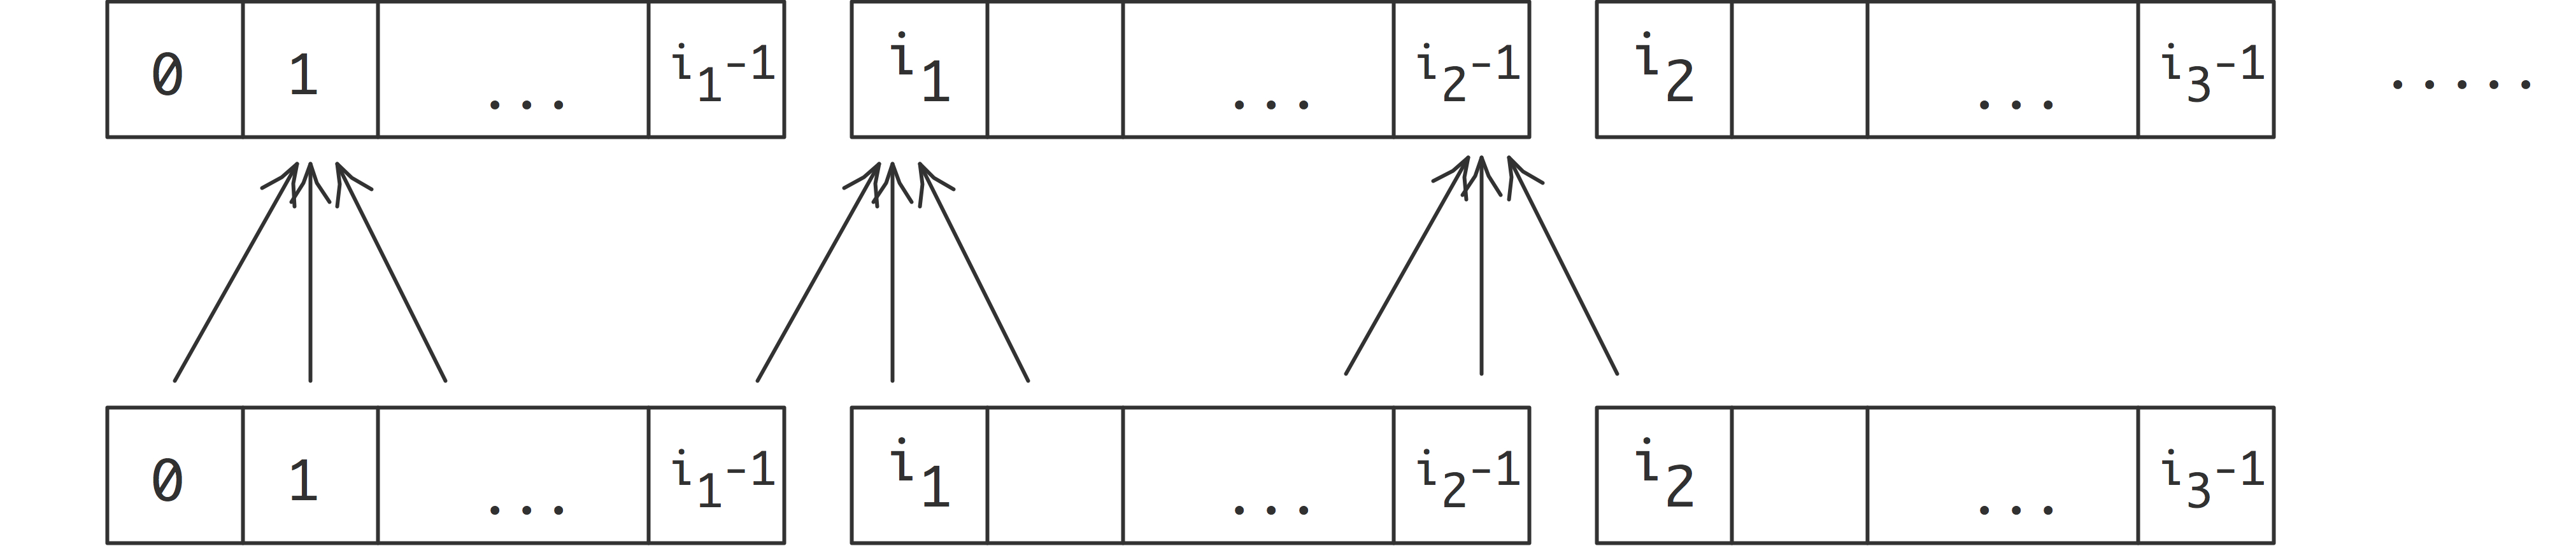
\includegraphics[scale=.09]{threepoint}
%%   \caption{Communication in an one-dimensional operation}
%%   \label{fig:3pt}
%% \end{figure}

We note:
\begin{itemize}
\item The data is one-dimensional, and we have a linear ordering of the processors.
\item The operation involves neighbouring data points, and we communicate
  with neighbouring processors.
\end{itemize}

Above you saw how you can use information exchange between pairs of processors
\begin{itemize}
\item using \indexmpishow{MPI_Send} and \indexmpishow{MPI_Recv}, if you are careful; or
\item using \indexmpishow{MPI_Sendrecv}, as long as there is indeed some sort of pairing of processors.
\end{itemize}
However, there are circumstances where it is not possible, not efficient, or simply not
convenient, to have such a deterministic setup of the send and receive calls.
%
\begin{figure}
  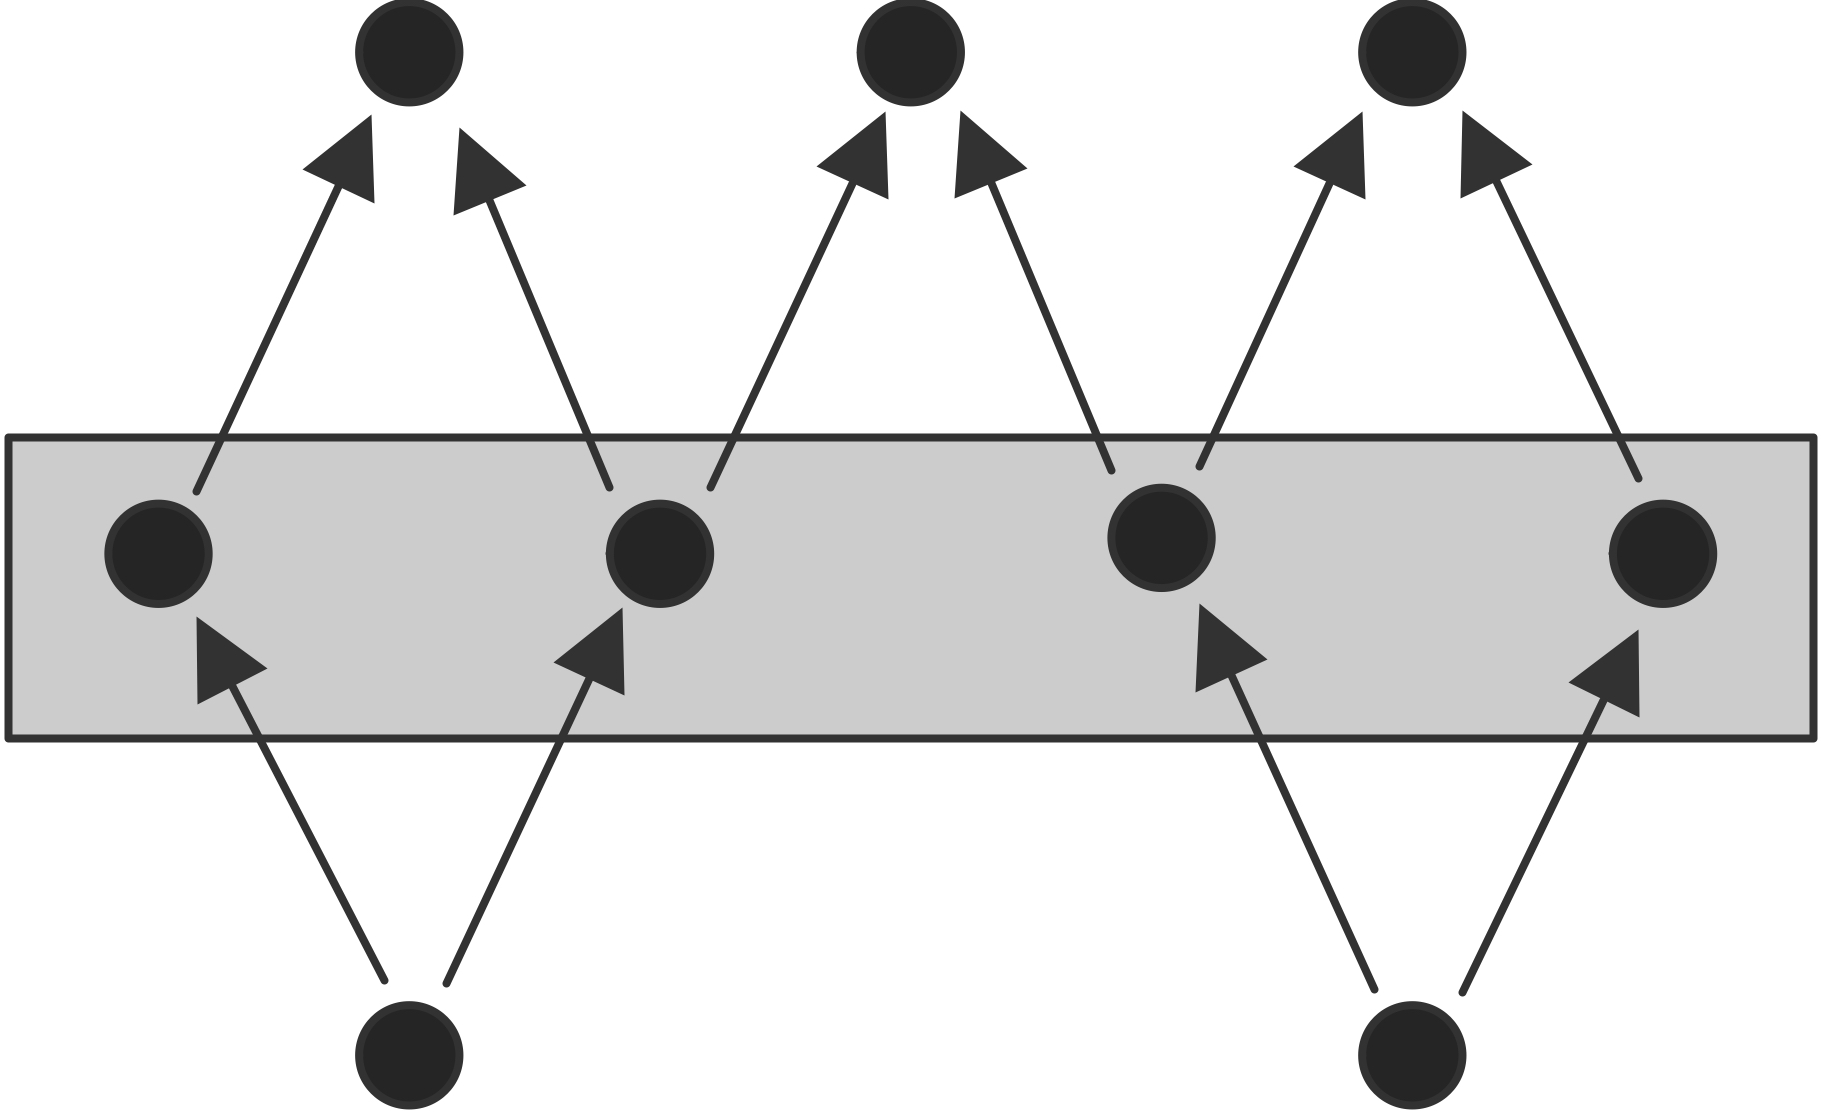
\includegraphics[scale=.1]{graphsend}
  \caption{Processors with unbalanced send/receive patterns}
  \label{fig:graphsend}
\end{figure}
%
Figure~\ref{fig:graphsend} illustrates such a case, where processors are
organized in a general graph pattern. Here, the numbers of sends and receive
of a processor do not need to match.

In such cases, one wants a possibility to state `these are the expected incoming
messages', without having to wait for them in sequence. Likewise, one wants to declare
the outgoing messages without having to do them in any particular sequence.
Imposing any sequence on the sends and receives is likely to run into the serialization
behaviour observed above, or at least be inefficient since processors will be
waiting for messages.

\Level 1 {Non-blocking communication}
\label{sec:nonblocking}
\index{communication!non-blocking|(textbf}

In the previous section you saw that blocking communication makes
programming tricky if you want to avoid \indexterm{deadlock} and performance
problems. The main advantage of these routines is that you have full
control about where the data is: if the send call returns
the data has been successfully received, and the send buffer can be used for
other purposes or de-allocated.  

\begin{figure}[ht]
  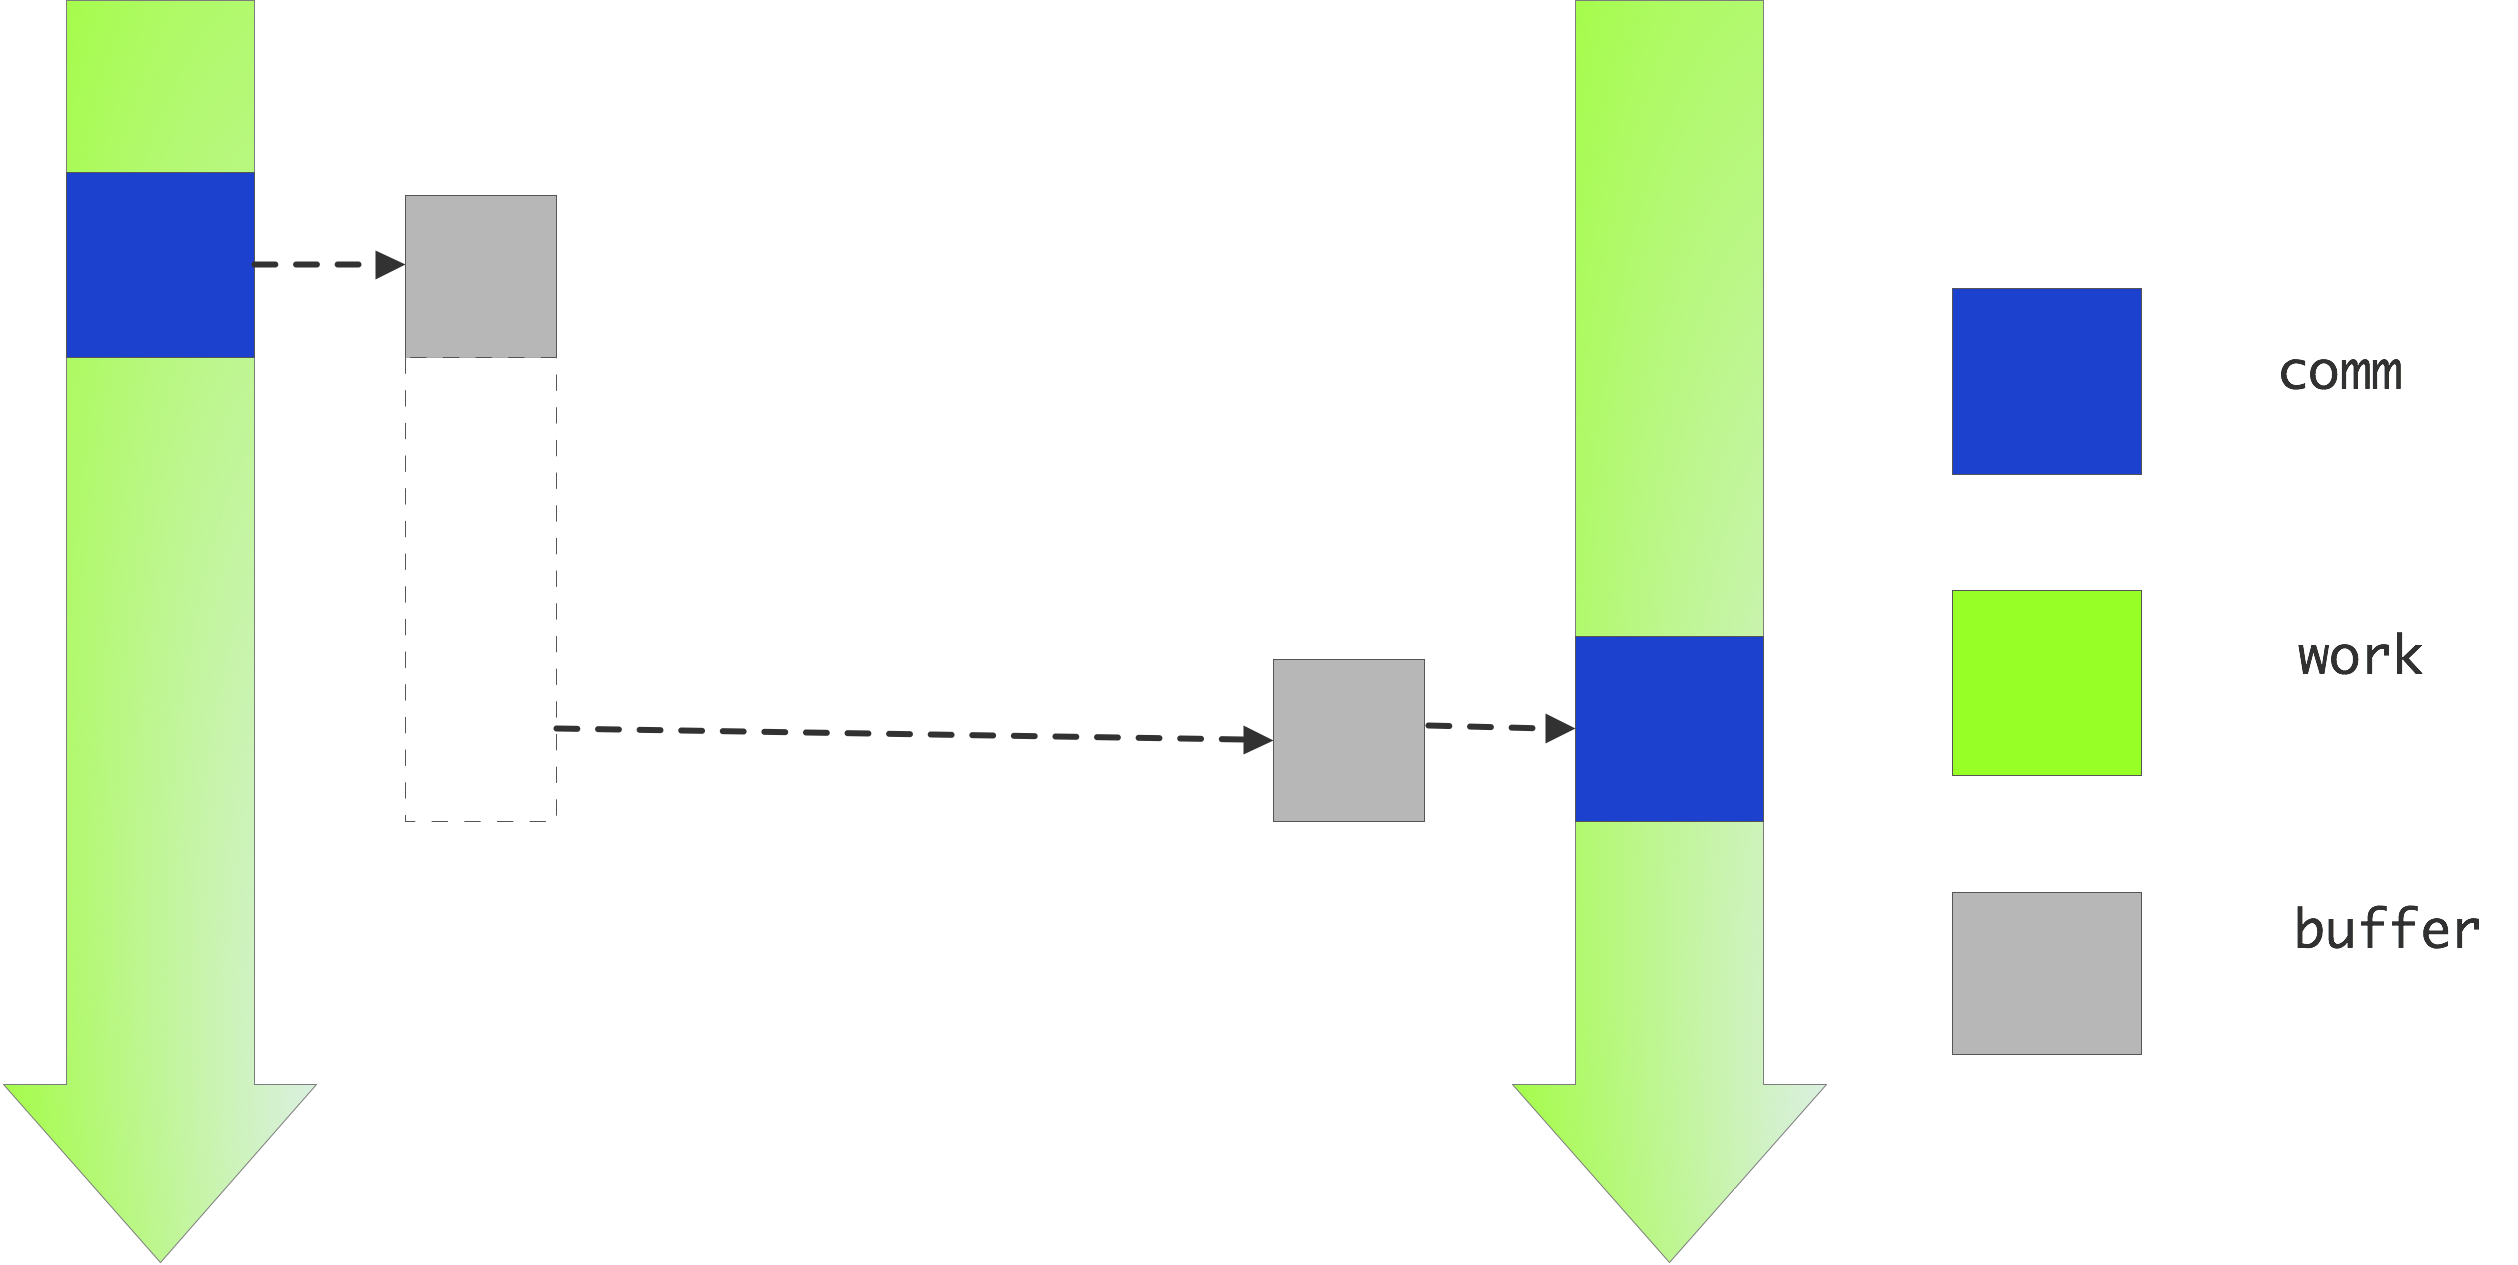
\includegraphics[scale=.1]{send-nonblocking}
  \caption{Non-blocking send}
  \label{fig:send-nonblocking}
\end{figure}

By contrast, the non-blocking calls \indexmpishow{MPI_Isend} and
\indexmpishow{MPI_Irecv} do not wait for their counterpart: in effect
they tell the runtime system `here is some data and please send it as
follows' or `here is some buffer space, and expect such-and-such data
to come'.  This is illustrated in figure~\ref{fig:send-nonblocking}.
Issuing the \n{Isend/Irecv} call is sometimes referred to as
\indexterm{posting} a send/receive.

\mpiRoutineRef{MPI_Isend}

\mpiRoutineRef{MPI_Irecv}

\Level 2 {Request completion}

From the definition of \indexmpishow{MPI_Isend}~/
\indexmpishow{MPI_Irecv}, you seen that non-blocking routinew yields
an \indexmpidef{MPI_Request} object. This request can then be used to
query whether the operation has concluded. You may also notice that
the \indexmpishow{MPI_Irecv} routine does not yield an
\indexmpishow{MPI_Status} object.  This makes sense: the status object
describes the actually received data, and at the completion of the
\indexmpishow{MPI_Irecv} call there is no received data yet.

\mpiRoutineRef{MPI_Request}

Waiting for the request is done with a number of routines. We first
consider \indexmpishow{MPI_Wait}. It takes the request as input, and
gives an \indexmpishow{MPI_Status} as output. If you don't need the
status object, you can pass \indexmpishow{MPI_STATUS_IGNORE}.

\mpiRoutineRef{MPI_Wait}

Note that the request is passed by reference, so that the wait routine
can free it.

\Level 2 {Buffer issues in non-blocking communication}

While the use of non-blocking routines prevents deadlock, it
introduces two new problems:
\begin{enumerate}
\item When the send call returns, the actual send may not have been executed,
  so the send buffer may not be safe to
  overwrite. When the recv call returns, you do not know for sure that
  the expected data is in it. Thus, you need a mechanism to make sure
  that data was actually sent or received.
\item With a blocking send call, you could repeatedly fill the send
  buffer and send it off.
\begin{lstlisting}
double *buffer;
for ( ... p ... ) {
   buffer = // fill in the data
   MPI_Send( buffer, ... /* to: */ p );
\end{lstlisting}
  To send multiple messages with non-blocking calls
  you have to allocate multiple buffers.
\begin{lstlisting}
double **buffers;
for ( ... p ... ) {
   buffers[p] = // fill in the data
   MPI_Send( buffers[p], ... /* to: */ p );
\end{lstlisting}
\end{enumerate}

\cverbatimsnippet[examples/mpi/c/irecvloop.c]{irecvloop}

\Level 2 {More wait calls}

MPI has two types of routines for handling requests; we will start
with the \indexmpishow{MPI_Wait...} routines. These
calls are blocking: when you issue
such a call, your execution will wait until the specified requests
have been completed. A~typical way of using them is:
\begin{lstlisting}
// start non-blocking communication
MPI_Isend( ... ); MPI_Irecv( ... );
// wait for the Isend/Irecv calls to finish in any order
MPI_Waitall( ... );
\end{lstlisting}

\mpiRoutineRef{MPI_Waitall}

If you don't need the status objects, you can pass
\indexmpishow{MPI_STATUSES_IGNORE}.

\begin{exercise}
  \label{ex:bucket-nonblock}
  Revisit exercise~\ref{ex:bucket-block} and consider replacing the
  blocking calls by non-blocking ones. How far apart can you put the
  \lstinline{MPI_Isend}~/ \lstinline{MPI_Irecv} calls and the
  corresponding \lstinline{MPI_Wait}s?
\end{exercise}

\Level 2 {Receive status of the wait calls}

The \lstinline{MPI_Wait...} routines have the \indexmpishow{MPI_Status}
objects as output.
If you are not interested in
the status information, you can use the values
\indexmpishow{MPI_STATUS_IGNORE} for \indexmpishow{MPI_Wait} and
\indexmpishow{MPI_Waitany},
or \indexmpishow{MPI_STATUSES_IGNORE} for \indexmpishow{MPI_Waitall}
and \indexmpishow{MPI_Waitsome}.

\begin{exercise}
  \label{ex:3ptnonblock}
  Now use nonblocking send/receive routines to implement
  the three-point averaging operation
  \[ y_i=\bigl( x_{i-1}+x_i+x_{i+1} \bigr)/3\colon i=1,\ldots,N-1 \]
  on a distributed array. (Hint: use \indexmpishow{MPI_PROC_NULL} at the ends.)
\end{exercise}

There is a second motivation for the \n{Isend/Irecv} calls:
if your hardware supports it, the communication can progress
while your program can continue to do useful work:
\begin{lstlisting}
// start non-blocking communication
MPI_Isend( ... ); MPI_Irecv( ... );
// do work that does not depend on incoming data
....
// wait for the Isend/Irecv calls to finish
MPI_Wait( ... );
// now do the work that absolutely needs the incoming data
....
\end{lstlisting}
This is known as \emph{overlapping computation and communication}, or
\indextermbusdef{latency}{hiding}.

Unfortunately, a~lot of this
communication involves activity in user space, so the solution would
have been to let it be handled by a separate thread. Until recently,
processors were not efficient at doing such multi-threading, so true
overlap stayed a promise for the future. Some network cards have
support for this overlap, but it requires a non-trivial combination of
hardware, firmware, and MPI implementation.

\begin{exercise}
  \label{ex:3ptnonblock-hide}
  Take your code of exercise~\ref{ex:3ptnonblock} and modify it to use
  latency hiding. Operations that can be performed without needing
  data from neighbours should be performed in between the
  \lstinline{MPI_Isend}~/ \lstinline{MPI_Irecv} calls and the
  corresponding \lstinline{MPI_Wait} calls.
\end{exercise}

\begin{remark}
  There is nothing special about a non-blocking or
  synchronous message. The \indexmpishow{MPI_Recv} call can match any of the
  send routines you have seen so far (but not \indexmpishow{MPI_Sendrecv}), and
  conversely a message sent with \indexmpishow{MPI_Send} can be received by \indexmpishow{MPI_Irecv}.
\end{remark}

\Level 2 {Asynchronous progress}
\label{sec:progress}

Above we saw that \n{Isend/Irecv} calls can overlap communication and
computation. 
However, for this to happen we need for the MPI
implementation to make
\indextermsub{asynchronous}{progress}: the message needs to make its way
through the network while the application is busy computing.
%
However, communication of this sort can 
typically not be off-loaded to the network card, so different
mechanisms are needed.

This can happen in a number of ways:
\begin{itemize}
\item Compute nodes may have a dedicated communications processor. The
  \indextermbus{Intel}{Paragon} was of this design; modern
  multicore processors are a more efficient realization of this idea.
\item The MPI library may reserve a core or thread for communications
  processing. This is implementation dependent; for instance,
  \indextermbus{Intel}{MPI} has a number of
  \indextermtt{I_MPI_ASYNC_PROGRESS_...} variables.
\item Absent such dedicated resources, the application can force MPI
  to make progress by occasional calls to a \indexterm{polling}
  routine such as \indexmpishow{MPI_Iprobe}.
\end{itemize}

A similar problem arises with passive target synchronization:
it is possible that the origin process may hang until 
the target process makes an MPI call.

\Level 2 {Wait and test calls}
\label{sec:waittest}

There are several wait calls: you can wait for a single request, all
outstanding requests, or any of the outstanding requests.

%\Level 3 {Wait for one request}

\indexmpishow{MPI_Wait} waits for a a single request. If you are
indeed waiting for a single nonblocking communication to complete,
this is the right routine. If you are waiting for multiple requests
you could call this routine in a loop.

\begin{lstlisting}
for (p=0; p<nrequests ; p++) // Not efficient!
  MPI_Wait(request[p],&(status[p]));
\end{lstlisting}

However, this would be inefficient if the first request is fulfilled
much later than the others: your waiting process would have lots of
idle time. In that case, use one of the following routines.

%\Level 3 {Wait for all requests}
  
\indexmpishow{MPI_Waitall} allows you to wait for a number of
requests, and it does not matter in what sequence they are
satisfied. Using this routine is easier to code than the loop above,
and it could be more efficient.

\mpiRoutineRef{MPI_Waitall}

%\Level 3 {Wait for any/some requests}

The `waitall' routine is good if you need all nonblocking
communications to be finished before you can proceed with the rest of
the program. However, sometimes it is possible to take action as each
request is satisfied. In that case you could use
\indexmpishow{MPI_Waitany} and write:

\begin{lstlisting}
for (p=0; p<nrequests; p++) {
  MPI_Waitany(nrequests,request_array,&index,&status);
  // operate on buffer[index]
}
\end{lstlisting}

Note that this routine takes a single status argument, passed by
reference, and not an array of statuses!

\mpiRoutineRef{MPI_Waitany}

Finally, \indexmpishow{MPI_Waitsome} is very much like \n{Waitany},
except that it returns multiple numbers, if multiple requests are
satisfied. Now the status argument is an array of \indexmpishow{MPI_STATUS}
objects.

Figure~\ref{fig:jump-nonblock} shows the trace of a non-blocking execution
using \indexmpishow{MPI_Waitall}.
\begin{figure}[ht]
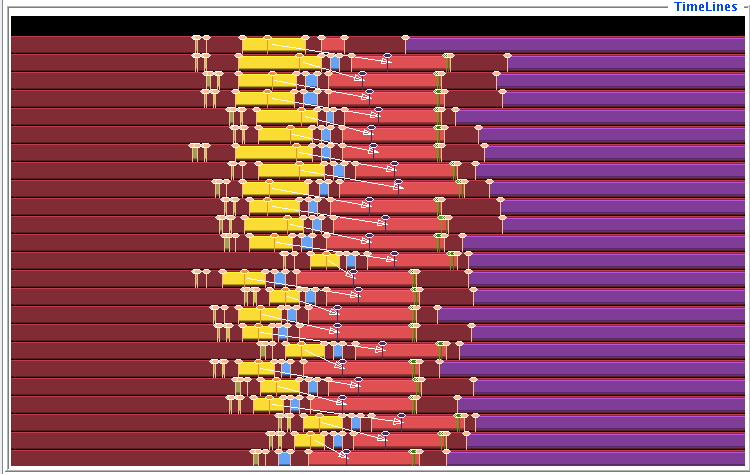
\includegraphics[scale=.4]{graphics/linear-nonblock}
\caption{A trace of a nonblocking send between neighbouring processors}
\label{fig:jump-nonblock}
\end{figure}

\Level 2 {Implementing polling with Waitany}

The \indexmpishow{MPI_Waitany} routine can be used to implement
\indexterm{polling}: occasionally check for incoming messages while
other work is going on.
%
\cverbatimsnippet[examples/mpi/c/waitforany.c]{waitforany}
%
\pverbatimsnippet{waitforanyp}
%
Each process except for the root does a blocking send; the root
posts \indexmpishow{MPI_Irecv} from all other processors, then loops
with \indexmpishow{MPI_Waitany} until all requests have come in. Use
\indexmpishow{MPI_SOURCE} to test the index parameter of the wait
call.

Note the \indexmpishow{MPI_STATUS_IGNORE} parameter: we know everything
about the incoming message, so we do not need to query a status object.
Contrast this with the example in section~\ref{sec:mpi-source}.

\begin{pythonnote}
  In python creating the array for the returned requests is somewhat
  tricky.
  %
  \pverbatimsnippet{irecvallp}  
\end{pythonnote}

\begin{fortrannote}
  The \n{index} parameter is the index in the array of requests,
  so it uses \emph{1-based indexing}\index{Fortran!1-based indexing}.
  \fverbatimsnippet{waitforany-f}
\end{fortrannote}

\Level 2 {Test: non-blocking request wait}
\label{sec:mpi-test}

The \n{MPI_Wait...} routines are blocking. Thus, they are a good solution if 
the receiving process can not do anything until the data 
(or at least \emph{some} data) is actually received.
The \indexmpishow{MPI_Test....} calls are themselves non-blocking: they
test for whether one or more requests have been
fullfilled, but otherwise immediately return.
This can be used in the
\indexterm{manager-worker model}: the manager process creates tasks, and
sends them to whichever worker process has finished its work.
(This uses a receive from \indexmpishow{MPI_ANY_SOURCE}, and a
subsequent test on the \indexmpishow{MPI_SOURCE} field of the receive status.)
While waiting for the workers, the manager can do useful work too,
which requires a periodic check on incoming message.

Pseudo-code:
\begin{lstlisting}
while ( not done ) {
  // create new inputs for a while
  ....
  // see if anyone has finished
  MPI_Test( .... &index, &flag );
  if ( flag ) {
    // receive processed data and send new
}
\end{lstlisting}

\mpiRoutineRef{MPI_Test}
\mpiRoutineRef{MPI_Testany}
\mpiRoutineRef{MPI_Testall}

\begin{exercise}
  Read section~\HPSCref{sec:pspmvp} and give pseudo-code for the
    distributed sparse matrix-vector product using the above idiom for
    using \n{MPI_Test...} calls. Discuss the advantages and
    disadvantages of this approach. The answer is not going to be
    black and white: discuss when you expect which approach to be
    preferable.
\end{exercise}

\Level 2 {More about requests}

Every non-blocking call allocates an \indexmpishow{MPI_Request}
object. One effect of the various \indexmpishow{MPI_Wait...} calls is
to deallocate these objects. Thus, it is wise to issue wait calls even
if you know that the operation has succeeded. For instance, if all
receive calls are concluded, you know that the corresponding send
calls are finished and there is no strict need to wait for their
requests. However, omitting the wait calls would lead to a memory
leak.

Another way around this is to call \indexmpishow{MPI_Request_free},
which sets the request variable to \indexmpishow{MPI_REQUEST_NULL},
and marks the object for deallocation after completion of the
operation.

Note that \indexmpishow{MPI_Test...} routines also deallocates the
request object, setting the handle to \indexmpishow{MPI_REQUEST_NULL},
but \indexmpishow{MPI_Request_get_status} does not alter the request
handle or object.

\index{communication!non-blocking|)}


